\part{Protocol Transition Systems and Serializability}

\chapter{Protocol Transition Systems}
\label{sec-trs}

The very first task to verify cache-coherence protocols in a theorem prover is to define an underlying state-transition system formally.
Formalization of such a system typically consists of its formal syntax and semantics.
Additionally, if we want to verify a program defined in the system, a correctness criterion should be established as well.
In this chapter, we provide the formal definition of the state-transition system for cache-coherence protocols, called \emph{protocol transition systems}.

\section{Cache-Coherence Protocol as a Message-Passing System}
\label{sec-cc-as-mp}

In a cache-coherence protocol, cache objects in a system communicate with each other via \emph{messages}.
Such communication is asynchronous in that a sender (a cache object) sends a message to a channel first, and a receiver handles it later.
Here the notion of a channel is logical, but the actual hardware implementation may use various hardware components (\eg{} finite-capacity FIFOs or buses) that can simulate it.
The hardware implementation of communication channels will be explained in detail later in \autoref{sec-comp-syn}.

The correctness proof of a cache-coherence protocol heavily relies on the formalization of a message-passing system.
An incorrect formalization can lead to a protocol unprovable.
It is also a part of trusted computing base (TCB); one must read through the formalization and be convinced that it is fair.
The formalization of a message-passing system varies by its purpose.
For instance, in order to reason about software distributed protocols, one may want to add Byzantine fault models~\cite{byzantine} to the formalization.

A cache-coherence protocol also requires its specific assumptions on top of a message-passing system.
First of all, each channel should be ordered; it is used practically, and the correctness of the protocol depends on it.
Also, each channel cannot be accessed twice in a single state-transition cycle, \eg{} one cannot push two different messages to a channel in the same cycle.
This constraint is also due to the practical implementations of an ordered channel; considering a channel as a black-box circuitry, there is usually a single ``wire'' to push a new element to the channel, thus accessing it twice (through the wire) is not possible.

Last but foremost, a conventional message-passing system assumes that it is fair to reason a single state transition (by a single object) at a time.
In other words, while multiple objects make their local state transitions by consuming and generating messages in actual execution, it is still fine to assume that a state-transition step is made by a single object.
This assumption is powerful especially in verification, since without it there would be exponential number of cases to consider for a state transition.
We certainly want to utilize the assumption in reasoning cache-coherence protocols.
Fortunately, a convenient concept has been developed in rule-based hardware description languages (RHDLs) such as Bluespec SystemVerilog~\cite{bluespec}, called ``one-rule-at-a-time semantics.''
Our cache-coherence protocol descriptions will be rule-based, and thus our formalization of the underlying system will assume that rules are executed atomically, even when multiple rules are executed at the same time.
It is worth noting that the one-rule-at-a-time semantics has been used in designing/verifying hardware components~\cite{Murali:2015,Dave:2005,Dave:2007} and formalized~\cite{fesi,kami,koika}.

\section{Formal Definition of Protocol Transition Systems}

Now we provide the formal syntax and semantics for message-passing-based state-transition systems, called \emph{protocol transition systems}.

\subsection{Syntax}
\label{sec-syntax}

\paragraph{Notations}
Throughout the thesis, we will use several notations for lists (sequences) and finite maps.
An overline (\eg{} $\listof{l}$) denotes a list.
$\llistof{l}$ denotes a list of lists.
$\listnil{}$, $(\listcons{\listof{l}}{e})$, $(\listapp{\listof{l_1}}{\listof{l_2}})$, $(\listsub{\listof{l_1}}{\listof{l_2}})$, and
$(\listdisj{\listof{l_1}}{\listof{l_2}})$ denote nil, single-element append, general append, subtraction, and disjointness of lists, respectively.
We use the same operation $(+)$ for the single-element and general append.
$\listconcat{\llistof{l}}$ flattens the list of lists $\llistof{l}$ with repeated concatenation.
$\sizeof{\listof{l}}$ is the length of a list.

Regarding a list of key-value pairs as a finite map, we override notations for lists.
For example, $(\mapupds{M}{\listof{l}})$ updates multiple key-value pairs in a finite map $M$.
Moreover, we overload the same operation $(\mapupd{M}{k}{v})$ for a single update for simplicity.

We will use $\tuple{\cdot}$ to denote a struct and use a name (\eg{} $s.\textsf{fd}$) to access a field value.
$(\listof{s.\textsf{fd}})$ will be used as a shorter notation for $(\textsf{List.map}\ (\lambda s.\; s.\textsf{fd})\ \listof{s})$.

\begin{figure}[t]
  \centering
  \begin{tabular}{|c|}
    \hline
    \begin{math}
      \begin{array}{rl}
        \textrm{ID} & \msgid{} \in \hidxt{} \\
        \textrm{Value} & \msgval{} \in \hvaluet{} \\
        \textrm{Message} & m ::= \msgbuild{\msgty}{\msgid}{\msgval} \in \hmsgt{} \triangleq \boolt \ast \hidxt \ast \hvaluet \\
        \textrm{Index} & i \in \hidxt{}\ \textrm{(for channels, objects, etc.)} \\
        \textrm{Channel Index \& Message} & im ::= \idmbuild{i}{m} \in \hidmt \triangleq \hidxt \ast \hmsgt \\
        \textrm{Object state} & o \in \hostt{} \\
        \textrm{Rule precondition} & \ruleprec{} \in \hostt \times \listtof{\hidmt} \to \propt \\
        \textrm{Rule transition} & \ruletrs{} \in \hostt \times \listtof{\hidmt} \to \hostt \times \listtof{\hidmt}\\
      \end{array}
    \end{math}\\
    \hline
    \begin{math}
      \begin{array}{rl}
        \textrm{Rule} & r ::= \tuple{i, \ruleprec{}, \ruletrs{}} \\
        \textrm{Object} & O ::= \tuple{i, \objInit{o}, \listof{r}} \\
        \textrm{System} & S ::= \hsyss{\listof{O}}{i} \\
      \end{array}
    \end{math}\\
    \hline
  \end{tabular}
  \caption{Protocol transition system}
  \label{fig-trs-system}
\end{figure}

\hemiola{} uses formal protocol transition systems as an underlying basis for reasoning about cache-coherence protocols.
\autoref{fig-trs-system} explains what such systems are.
A \emph{message} $m$ is a communication unit, consisting of a Boolean message type, a message ID, and a value.
A message type is false (true) for a request (response), respectively.
A message ID is an enumeration of message kinds.
We use \emph{value} to refer to each line in a cache or a memory.
Note that a struct sometimes has an \emph{index} to distinguish it from the other components.
A pair \idmbuild{i}{m} is used to represent a message $m$ residing in a channel with an index $i$.

Rules make local state transitions within an object.
A rule $r$ is a struct composed of its rule index, a precondition (\ruleprec{}), and a transition function (\ruletrs{}).
Each rule has a unique index within an object.
A precondition \ruleprec{} takes two arguments, a current object state and input messages (as a list of pairs \idmbuild{i}{m}), and decides whether the rule can be executed or not with the current state.
A transition function takes the same arguments but returns the next object state and output messages (also as a list of \idmbuild{i}{m}).
Note that our formalization of the protocol transition system is shallowly embedded in Coq, \eg{} precondition and transition definitions use native Coq function types.

An object $O$ contains its object index (unique within a system), an initial state ($\objInit{o}$), and rules (\listof{r}) that make local state transitions within the object.
The highest-level component is a system $S$, which contains information about objects and channels.
It consists of objects (\listof{O}) and channel indices for internal messages (\hsysIn{i}), external inputs (\hsysRq{i}), and external outputs (\hsysRs{i}).
The definition is general in that any object can access any channel in the system, just by mentioning the channel index in a state transition.
It is necessary to distinguish between internal and external channels, in order to define external behaviors of the system, \ie{} the interface of the cache-coherence protocol with processor cores, which will be explained in \autoref{sec-semantics}.

\subsection{Semantics}
\label{sec-semantics}

\subsubsection{State-transition steps}

\begin{figure}[t]
  \centering
  \begin{tabular}{|c|}
    \hline
    \multicolumn{1}{|l|}{\textbf{Types:}} \\
    \begin{tabular}{lr}
      $\textrm{Message States}\ \ M \in \hidxt{} \to \listtof{\hmsgt}$ &
      $\textrm{State}\ \ s \in \hstt{} ::= \tuple{\listof{o}, M}$ \\
      \multicolumn{2}{l}{$\textrm{Label}\ \ l ::= \lblEmpty{}\; |\; \lblIns{\listof{im}}\; |\; \lblOuts{\listof{im}}\; |\; \lblInt{\idxOf{O}}{\idxOf{r}}{\listof{im}}{\listof{im}}$} \\
    \end{tabular}\\
    \multicolumn{1}{|l|}{\textbf{Step:}} \\
    \begin{math}
      \begin{array}{c}
        \inference[StepSilent:]{}{\semstep{S}{s}{\lblEmpty{}}{s}}\bigskip\\
        \inference[StepIns:]{\listof{im} \neq \listnil
          & \listof{\idxOf{im}} \subseteq \hsysRqA{S}}{\semstep{S}
          {\hst{\listof{o}}{M}}
          {\lblIns{\listof{im}}}
          {\hst{\listof{o}}{\enqMsgs{M}{\listof{im}}}}}\bigskip \\
        \inference[StepOuts:]{\listof{im} \neq \listnil
          & \listof{im} \subseteq \heads{M}
          & \listof{\idxOf{im}} \subseteq \hsysRsA{S}}{\semstep{S}
          {\hst{\listof{o}}{M}}
          {\lblOuts{\listof{im}}}
          {\hst{\listof{o}}{\deqMsgs{M}{\listof{im}}}}}\bigskip \\
        \inference[StepInt:]{S = \hsyss{\listof{O}}{i}
          & O \in S.\listof{O}
          & r \in O.\listof{r}\smallskip \\
          \midxIns{im} \subseteq \hsysInA{S} \cup \hsysRqA{S}
          & \listof{o}[\idxOf{O}] = o_1
          & \msgIns{im} \subseteq \heads{M}\smallskip \\
          \rprecOf{r}\enspace (o_1, \msgIns{im})
          & \rtrsOf{r}\enspace (o_1, \msgIns{im}) = (o_2, \msgOuts{im})\smallskip \\
          \midxOuts{im} \subseteq \hsysInA{S} \cup \hsysRsA{S}
          & \disj{\midxIns{im}}{\midxOuts{im}}}{\semstep{S}
          {\hst{\listof{o}}{M}}
          {\lblInt{\idxOf{O}}{\idxOf{r}}{\msgIns{im}}{\msgOuts{im}}}
          {\hstm{\mapupd{\listof{o}}{\idxOf{O}}{o_2}}{\enqMsgs{\deqMsgs{M}{\msgIns{im}}}{\msgOuts{im}}}}}\medskip \\
      \end{array}
    \end{math}\\
    \hline
  \end{tabular}
  \caption{Step semantics in protocol transition systems}
  \label{fig-trs-semantics-steps}
\end{figure}

\autoref{fig-trs-semantics-steps} describes the semantics for state-transition steps in a protocol transition system.
A state transition (step) happens by a rule that takes input messages, makes an object-state transition, and generates output messages.
The semantics for a step is presented as a judgment \semstep{S}{s_0}{l}{s_1}, where $S$ is the system to execute, $s_0$ is a prestate, $s_1$ is a poststate, and $l$ is a label generated by the state transition.
The state of a system (in domain $\hstt{}$) is a pair of object states and message states.
Object states are represented in a finite map from object indices to object states.
Message states are also represented in a finite map from channel indices to ordered queues of messages.

From now on, we assume that all the input and output messages used in the step definitions do not share the same channel, \ie{} $(\nodup{\listof{\idxOf{im}}})$.
In other words, while taking inputs and generating outputs, each step case never accesses a channel twice.
As already mentioned in \autoref{sec-cc-as-mp}, this assumption is fair and practical in hardware.

Rule [StepSilent] represents the case where no state transition happens in the current step; an empty label (\lblEmpty{}) is generated in this case.
A system may accept input messages from the external world.
[StepIns] describes this case, where the external input messages (\listof{im}) should not be empty ($\listof{im} \neq \listnil$), and channels of the messages are valid ($\listof{\idxOf{im}} \subseteq \hsysRqA{S}$), \ie{} the input messages are all put to external-request channels.
An external-inputs label $(\lblIns{\listof{im}})$ is generated in this case.
[StepOuts] describes the opposite case, for output messages being released to the external world.
In this case, in addition to the [StepIns] case, each output message should be in the head (the first element) of its residing channel ($\listof{im} \subseteq \heads{M}$).

Lastly, [StepInt] deals with a state transition by a rule ($r$) in an object ($O$).
It nondeterministically chooses an object and a rule in the object, checks that the precondition holds ($r.p\enspace (o_1, \msgIns{im})$), and applies the transition to update the state of the system ($r.t\enspace (o_1, \msgIns{im}) = (o_2, \msgOuts{im})$).
An internal label ($\lblInt{\idxOf{O}}{\idxOf{r}}{\msgIns{im}}{\msgOuts{im}}$) is generated in this case, which records an object index, a rule index, input messages, and output messages.
Each input message should be from either an internal channel or an external-request one ($\midxIns{im} \subseteq \hsysInA{S} \cup \hsysRqA{S}$) and should be the first element of the channel ($\msgIns{im} \subseteq \heads{M}$).
On contrary to the input messages, each output message should be enqueued to either an internal channel or an external-response one ($\midxOuts{im} \subseteq \hsysInA{S} \cup \hsysRsA{S}$).
Lastly, the channels of the input and output messages should be disjoint to each other ($\disj{\midxIns{im}}{\midxOuts{im}}$).
Note that the semantics is based on ordered channels, so messages are \emph{enqueued} and \emph{dequeued} in each state-transition case.
We use notations $\enqMsgs{M}{\listof{im}}$ and $\deqMsgs{M}{\listof{im}}$ for such operations.

\begin{figure}[t]
  \centering
  \begin{tabular}{|c|}
    \hline
    \multicolumn{1}{|l|}{\textbf{Steps and behaviors:}} \\
    \begin{math}
      \arraycolsep=10pt
      \begin{array}{cc}
        \inference[StepsNil:]{}{\semsteps{S}{s}{\listnil{}}{s}}
        & \inference[StepsCons:]{\semsteps{S}{s_0}{\listof{l}}{s_1}
          & \semstep{S}{s_1}{l_1}{s_2}}{\semsteps{S}{s_0}{\listcons{\listof{l}}{l_1}}{s_2}}\medskip \\
      \end{array}
    \end{math}\\
    \begin{tabular}{c}
      \inference[Behavior:]{\semsteps{S}{\sysInit{S}}{\listof{l}}{s}}{\sembeh{S}{\behOf{\listof{l}}}}\medskip\\
    \end{tabular}\\
    \hline
  \end{tabular}
  \caption{Multiple transition steps and behaviors in protocol transition systems}
  \label{fig-trs-semantics-steps-beh}
\end{figure}

The step semantics is naturally lifted to one for multiple steps, as shown in \autoref{fig-trs-semantics-steps-beh}.
It is presented as a judgment $\semsteps{S}{s_0}{\listof{l}}{s_1}$, where $S$ is the system to execute, $s_0$ is a prestate, $s_1$ is a poststate, and $\listof{l}$ is a \emph{sequence of labels} generated by executions of the steps.
[StepsNil] serves the case where no state transitions happen, and no labels are generated in this case.
[StepsCons] is a natural inductive constructor that combines previous steps (\semsteps{S}{s_0}{\listof{l}}{s_1}) and a new one (\semstep{S}{s_1}{l_1}{s_2}).
The label by the new step is appended to the last of the label sequence of the previous steps.

Throughout the thesis, we will now call a sequence of labels a \emph{history}.
We say that a state $s$ is \emph{reachable} iff there is a history $\listof{l}$ such that $\semsteps{S}{\sysInit{S}}{\listof{l}}{s}$ holds, where $\sysInit{S}$ is the initial state of the system $S$, constructed by composing all initial object states.
We use a simpler notation $\semrch{S}{s}$ for reachable states.
We also say that a history $\listof{l}$ is \emph{legal} iff there is a state $s$ such that $\semsteps{S}{\sysInit{S}}{\listof{l}}{s}$ holds.
We write $\semleg{S}{\listof{l}}$ to assert that a history is legal.

\subsubsection{Behaviors and correctness}

A system $S$ has a behavior $\behOf{\listof{l}}$, denoted as \sembeh{S}{\behOf{\listof{l}}}, if there exists an execution of steps that generates $\listof{l}$, starting with the initial state of $S$ ([Behavior] in \autoref{fig-trs-semantics-steps-beh}).
Here the $\behOf{\cdot}$ operation filters out silent ($l_\epsilon$) and internal ($l_{\textrm{int}}$) labels so only the external parts remain.
We call such a sequence of labels a \emph{trace}.
In other words, a trace only consists of external-inputs and external-outputs labels.

Finally we define trace refinement as a notion of correctness in protocol transition systems:
\begin{definition}[Trace Refinement]
  A system $I$ (``implementation'') trace-refines another system $S$ (``specification''), written as $\refines{I}{S}$, iff every trace of $I$ is also a trace of $S$:
  \begin{displaymath}
    \refines{I}{S} \triangleq \forall \listof{t}.\; \sembeh{I}{\listof{t}} \to \sembeh{S}{\listof{t}}.
  \end{displaymath}
\end{definition}

Trace refinement is one of the well-known correctness criteria to claim that the external (observable) behavior of a given implementation is within the behavior boundary of the specification.
In other words, by proving trace refinement, we can say that the implementation does not go wrong in terms of the specification.

How do we prove trace refinement for a given implementation and a spec?
It is usually proven by establishing a \emph{simulation} relation between the implementation and the spec states:
\begin{definition}[Simulation]
  We call a relation between two states $(\sim): \hstt{} \times \hstt{} \to \propt{}$ a simulation between the systems $I$ and $S$ iff 1) the relation holds for the initial states and 2) a step in $S$ exists for every step in $I$, which generates the same external label and preserves the relation:
  \begin{displaymath}
    \begin{array}{rl}
      1) & \sysInit{I} \sim \sysInit{S},\\
      2) & \forall s_0, s_1, l.\; \semstep{I}{s_0}{l}{s_1} \to \forall t_0.\; s_0 \sim t_0 \to \exists t_1.\; \semstep{S}{t_0}{l}{t_1} \wedge s_1 \sim t_1.
    \end{array}
  \end{displaymath}
\end{definition}

It is also well-known that simulation directly implies trace refinement~\cite{equivalence}, which is proven simply by induction on state-transition steps:
\begin{theorem}[Simulation implies trace refinement]
  If there is a simulation $(\sim)$ between two systems $I$ and $S$, then \refines{I}{S}.
\end{theorem}

\chapter{Serializability in Protocol Transition Systems}
\label{sec-sz-def}

Serializability~\cite{sz1,sz2} is a celebrated notion of concurrency correctness that originated with databases and distributed systems.
While each transaction in a system affects multiple values, serializability guarantees that concurrent execution of such transactions is correct in that the effect (state change) is the same as if the transactions were executed separately in sequence.
In this section, we provide the formal definition of serializability on top of a protocol transition system and explain how it eases the burden of designing and proving conventional invariants.

\section{Cache-Coherence Protocol as a Distributed Protocol}

We already explored in \autoref{sec-nutshell} with a concrete example that the cache objects in a cache-coherent memory system handle multiple requests from the processor cores concurrently, in a distributed way.
We also learned that transactions to handle such requests are interleaved, so it is crucial in designing and proving a cache-coherence protocol to ensure safe interleavings.

A very well-known approach to ensuring safe interleavings is to prove \emph{noninterference}, which basically claims that no other state transitions spuriously affect state relevant to an ongoing transaction.
Not constrained to the cache-coherence protocols, noninterference has been developed and employed in verifying various computer systems including concurrent software and distributed systems.

Model checkers have always been in favor of employing noninterference lemmas.
The lemmas are often described explicitly by the user (guided by intuition) or discovered automatically (typically guided by counterexamples).
The established style of noninterference reasoning, though, has an inherent weakness: it requires explicit lemma statements per-protocol.
Another issue is that even though these lemmas are stated and proven, it is hard to be sure if the lemmas are enough to resolve all possible interleavings in the system.

Another well-known approach is to prove \emph{serializability}, which claims that the overall state transition of any interleaved transactions can be interpreted as if they are executed serially, \ie{} \emph{atomically in some order with no interleaving}.
Serializability has been mainly developed and used in database systems and software distribued systems.
Regarding a cache-coherence protocol as a distributed protocol, one of the main topics of this thesis is to demonstrate that serializability can be also employed to prove the protocol.
To our knowledge, the notion of serializability has not been used to provide a formal correctness proof of a cache-coherence protocol.
Instead of stating noninterference lemmas coupled to each protocol, which is a conventional approach to the verification of cache-coherence protocols, in \hemiola{} we try to find general conditions that ensures serializability, \emph{extracted and abstracted} from practical protocols, so the conditions can apply to various protocols.

\section{From Atomic Histories to Serializability}

In order to obtain the formal definition of serializability, we should define each basic term first -- transactions, sequential executions, etc.
In this section, we provide all the formal definitions required to define serializability, starting with atomic histories.

\subsection{Atomic histories}

\begin{figure}[t]
  \centering
  \begin{subfigure}[b]{\columnwidth}
    \centering
    \begin{tabular}{|c|}
      \hline
      \begin{math}
        \begin{array}{c}
          \inference[AtomicStart:]{}{\atomicLong{\listof{\amsgi{im}}}{\listsingle{\lblInt{\idxOf{O}}{\idxOf{r}}{\listof{\amsgi{im}}}{\listof{\amsge{im}}}}}{28}{\listof{\amsge{im}}}}\\[25pt]
          \inference[AtomicCont:]{\atomic{\listof{\amsgi{im}}}{\listof{l}}{\listof{\amsge{im}}}
            & \msgIns{n} \neq \listnil
            & \msgIns{n} \subseteq \listof{\amsge{im}}}{\atomicLong{\listof{\amsgi{im}}}{\listcons{\listof{l}}{\lblInt{\idxOf{O}}{\idxOf{r}}{\msgIns{n}}{\msgOuts{n}}}}{28}{(\listapp{\listsub{\listof{\amsge{im}}}{\msgIns{n}}}{\msgOuts{n}}})} \\[25pt]
        \end{array}
      \end{math}\\
      \hline
    \end{tabular}
    \caption{Atomic histories}
    \label{fig-atomic-hst}
  \end{subfigure}\medskip\\
  \begin{subfigure}[b]{\columnwidth}
    \centering
    \begin{tabular}{|c|}
      \hline
      \begin{math}
        \begin{array}{cc}
          \begin{array}{c}
            \inference[TrsSilent:]{}{\trsn{S}{\listsingle{\lblEmpty{}}}} \\[10pt]
            \inference[TrsIns:]{}{\trsn{S}{\listsingle{\lblIns{\listof{im}}}}} \\[10pt]
            \inference[TrsOuts:]{}{\trsn{S}{\listsingle{\lblOuts{\listof{im}}}}} \\[15pt]
          \end{array} &
          \begin{array}{l}
            \textrm{\footnotesize TrsAtomic:} \\
            \inference[]{\extatomic{S}{\listof{\amsgi{im}}}{\listof{l}}{\listof{\amsge{im}}}}{\trsn{S}{\listof{l}}}
          \end{array} \\
        \end{array}
      \end{math}\\
      \hline
    \end{tabular}
    \caption{Transactions}
    \label{fig-transaction}
  \end{subfigure}
  \caption{Atomic histories and transactions in protocol transition systems}
  \label{fig-atomic-trs}
\end{figure}

\autoref{fig-atomic-trs} provides basic definitions of atomic histories and transactions.
A history $h$ is \emph{atomic} iff it satisfies the predicate $(\atomic{\listof{\amsgi{im}}}{h}{\listof{\amsge{im}}})$ with \emph{initial messages} $\listof{\amsgi{im}}$ and \emph{live messages} $\listof{\amsge{im}}$.
[AtomicStart] initializes a history with an internal label.
[AtomicCont] inductively adds a label to an atomic history, where the input messages of the new label \emph{should be from the live messages of the previous atomic history}.
A shorter notation $\atomicShort{h}$ will be used when $\listof{\amsgi{im}}$ and $\listof{\amsge{im}}$ are clear from context.

\begin{figure}[t]
  \centering
  \begin{tabular}{c}
    \begin{tikzpicture}
      \pic at (0, 0) {skeleton-pcce1={$P$}{$C_1$}{$C_2$}};
      % C_1 external
      \pic at (0, 0) {skeleton-midx-e1};
      \node[label={[label distance=-6pt,myred]left:{\sf\small rqWr}},color=myred] at (-1.6, -2.05) {$\bullet$};
      % Between P and C_1
      \pic at (0, 0) {skeleton-midx-pc1};
      \node[label={[label distance=-6pt,myred]left:{\sf\small rqM}},color=myred] at (-1, -0.7) {$\bullet$};
      % Between P and C_2
      \pic at (0, 0) {skeleton-midx-pc2};
      \node[label={[label distance=-9pt,myred]below left:{\sf\small rsI}},color=myred] at (0.8, -0.7) {$\bullet$};
      \node[label={[label distance=-9pt,myred]above right:{\sf\small rqI}},color=myred] at (1, -0.7) {$\bullet$};

      % Curves
      \draw [->,color=myred] (-2.2, -1.85) to[out=90,in=-110] node[left=3pt] {$r_1$} (-1.6, -0.95);
      \draw [->,color=myred] (-1.6, -0.45) to[out=70,in=120,distance=1.3cm] node[above] {$r_2$} (1.3, -0.2);
      \draw [->,color=myred] (1.45, -0.7) to[out=-50,in=-50,distance=1.7cm] node[below] {$r_3$} (0.5, -1.2);
    \end{tikzpicture}\\
    \hline
    \begin{math}
      \begin{array}{rl}
        h \triangleq & [\lblInt{\idxOf{C_1}}{\idxOf{r_1}}{\listsingle{(1, {\sf rqWr})}}{\listsingle{(3, {\sf rqM})}};\\
          & \lblInt{\idxOf{P}}{\idxOf{r_2}}{\listsingle{(3, {\sf rqM})}}{\listsingle{(8, {\sf rqI})}};\\
          & \lblInt{\idxOf{C_2}}{\idxOf{r_3}}{\listsingle{(8, {\sf rqI})}}{\listsingle{(7, {\sf rsI})}}]\\
      \end{array}
    \end{math}
  \end{tabular}
  \caption{An example of an atomic history}
  \label{fig-ex-atomic-history}
\end{figure}

\autoref{fig-ex-atomic-history} presents an example of an atomic history.
$h$ is generated by executions of three rules, $r_1 \in \hobjrules{C_1}$, $r_2 \in \hobjrules{P}$, and $r_3 \in \hobjrules{C_2}$.
Rule $r_1$ takes an input message $(1, \textsf{rqWr})$ (from the channel with index $1$) as an initial message of the history.
Rule $r_2$ takes $(3, \textsf{rqM})$, the output message from $r_1$.
Finally, $r_3$ takes $(7, \textsf{rqI})$, the output message from $r_2$.
Summing up all the rule executions, by the definition of an atomic history we get the predicate $\atomic{\listsingle{(1,\textsf{rqWr})}}{h}{\listsingle{(7,\textsf{rsI})}}$.
This example shows that an atomic history intuitively captures a \emph{transaction flow} triggered by the initial messages.
Note that an atomic history does not need to be a completed transaction.
The history $h$ in the example is not completed, in the sense that the live message ($\textsf{rsI}$) is not a response sent on an external channel.

We call a history \emph{externally atomic} if initial messages are external requests ($\listof{\idxOf{\amsgi{m}}} \subseteq \hsysRqA{S}$), denoted as $(\extatomic{S}{\listof{\amsgi{im}}}{h}{\listof{\amsge{im}}})$.
We sometimes use the shorter notation \extatomicShort{S}{h} for some \listof{\amsgi{im}} and \listof{\amsge{im}}.
The history $h$ in the example is externally atomic, satisfying a predicate \extatomic{S}{\listsingle{(1,\textsf{rqWr})}}{h}{\listsingle{(7,\textsf{rsI})}}, since the initial message $(1, \textsf{rqWr})$ is an external request (from a processor core attached to $C_1$).
An externally atomic history records the way the system responded to some set of messages received from the outside world.

\subsection{Transactions}

Transactions are the next level of abstraction, presented in \autoref{fig-transaction}.
A transaction is either a single silent label ([TrsSilent]), a single external inputs label ([TrsIns]), a single external outputs label ([TrsOuts]), or an externally atomic history ([TrsAtomic]).
In other words, the permitted atomic execution steps, in this transactional semantics, are arrival of new messages from the outside world, release of messages to the outside world, or uninterrupted execution of an atomic history.
We denote by $\trsn{S}{h}$ that $h$ is a transaction in $S$.

Note that an external-inputs label and an atomic history are regarded as separate transactions.
In other words, accepting an external request (or releasing an external response) is regarded as a transaction separated from the atomic history handling the request (generating the response), respectively.
This design choice gives more serializable histories in a given system, where the property is still meaningful enough to use it to verify distributed protocols.
We will see why this relaxed definition is a better choice right in the next section (\autoref{sec-seq-sz}).

\subsection{Sequential histories and serializability}
\label{sec-seq-sz}

With a clear notion of transactions, we can easily define sequential histories and serializability.

\begin{definition}[Sequential Histories and Serializability]
  \label{def-seq-sz}\mbox{}\vspace{-8pt}\\
  \begin{enumerate}[leftmargin=*]
  \item A history $h$ is \emph{sequential} iff the history is a concatenation of transactions:
    \begin{displaymath}
      \hseq{S}{h} \triangleq \exists\, \listof{t}.\; (\forall t \in \listof{t}.\; \trsn{S}{t}) \wedge h = \listconcat{\listof{t}}.
    \end{displaymath}
  \item A legal history $h$ is \emph{serializable} in the system $S$ iff there exists a sequential history that reaches the same state:
    \begin{align*}
      \hsrzl{S}{h} \triangleq\; & \forall s.\; \semsteps{S}{\sysInit{S}}{h}{s} \to\\
      & \exists\, h_{\textrm{seq}}.\; \hseq{S}{h_{\textrm{seq}}} \wedge \semsteps{S}{\sysInit{S}}{h_{\textrm{seq}}}{s}.
    \end{align*}
  \item A system $S$ is \emph{serializable} iff every legal history is serializable:
    \begin{displaymath}
      \hsrz{S} \triangleq \forall h.\; \hsrzl{S}{h}.
    \end{displaymath}
  \end{enumerate}
  \label{def-sz}
\end{definition}

Suppose that an object $C$ in a system $S$ takes two external requests, say $\textsf{rq}_1$ and $\textsf{rq}_2$, in-order from the same channel and finishes handling $\textsf{rq}_2$ earlier than $\textsf{rq}_1$.
Even if $C$ should start handling $\textsf{rq}_1$ first because the channel is ordered, this case may happen when $\textsf{rq}_1$ requires further treatment by other objects while $C$ can take $\textsf{rq}_2$ and respond immediately to the corresponding external channel.
We may have the following legal history $h$ in $S$ for this kind of scenario:
\begin{displaymath}
  h = \listcons{{\color{myred}\lblIns{\listsingle{(i_{\textrm{rq}},\textsf{rq}_1)}}}}{\listcons{{\color{myblue}\lblIns{\listsingle{(i_{\textrm{rq}},\textsf{rq}_2)}}}}{\listapp{h_a}{\listcons{{\color{myblue}\lblOuts{\listsingle{(i_{\textrm{rs}},\textsf{rs}_2)}}}}{{\color{myred}\lblOuts{\listsingle{(i_{\textrm{rs}},\textsf{rs}_1)}}}}}}},
\end{displaymath}
where $i_{\textrm{rq}}$ (and $i_{\textrm{rs}}$) is the external-request (external-response) channel, respectively.
If we had not separated the external labels from an atomic history and regard the combined history as a transaction, then we cannot sequentialize $h$, \ie{} separating the {\color{myred}red} and {\color{myblue}blue} transactions, thus $h$ is not serializable.
However, it is still meaningful if we can just sequentialize the internal processes of $\textsf{rq}_1$ and $\textsf{rq}_2$ (presented as $h_a$) to have two separated atomic histories.
The next section will explain how we benefit from this serializability definition.
Lastly, note that this relaxed definition is still safe in that it does not require preserving the order of the trace.

\section{Predicate Messages in Atomic Histories}
\label{sec-pred-msg}

Now we discuss how to exploit our notion of serializability: how does it help prove trace refinement between an implementation and its spec?
There is a clear gap between two notions, serializability and trace refinement: the former only deals with \emph{reachable states}, whereas the latter only deals with \emph{behaviors}.
However, we can bridge the gap by using serializability to help prove \emph{invariants} (which only concern reachable states), since a simulation -- which implies trace refinement -- proof usually requires a number of invariants of the implementation.

We start by defining a conventional notion of an invariant:
\begin{definition}[Invariants]
  We call $\mathcal{I}: \hstt{} \to \propt{}$ an \emph{invariant} over a system $S$ if $\mathcal{I}$ holds for all reachable states, \ie{} $\forall s.\; \semrch{S}{s} \to \mathcal{I}(s)$.
\end{definition}

In proving the correctness of a distributed protocol, it is quite common to state an invariant like ``some important property holds whenever the system includes a certain message in a certain channel.''
We call such an invariant a \emph{predicate message}, formally defined as following:
\begin{definition}[Predicate Messages]
  A predicate message, denoted as \spredmsg{S}{im}{P}, is an invariant over a system $S$ that additionally requires $im$, a pair of a residing channel and a message, to be in the system:
  \begin{displaymath}
    \spredmsg{S}{im}{\mathcal{I}} \triangleq \forall s.\; \semrch{S}{s} \to im \in s.M \to \mathcal{I}(s).
  \end{displaymath}
  \label{def-pred-msg}
\end{definition}

We will write just \predmsg{im}{\mathcal{I}} when the system $S$ is clear from context.
We will use an even-shorter version \predmsg{m}{\mathcal{I}} when the residing channel is not ambiguous.
The same notation \predmsg{\msgid{}}{\mathcal{I}} will be used most commonly to define a predicate message that holds for every message with a given ID (\msgid{}) with the clear residing channel.

\begin{figure}[h]
  \centering
  \begin{tikzpicture}
    \pic at (0, 0) {skeleton-pcce1={$P$}{$C_1$}{$C_2$}};
    % C_1 external
    \pic at (0, 0) {skeleton-midx-e1};
    \node[label={[label distance=-6pt,myred]right:{\msgsfsm{rsWr}}},color=myred] at (-1.6, -2.25) {$\bullet$};
    % Between P and C_1
    \pic at (0, 0) {skeleton-midx-pc1};
    \node[label={[label distance=-11pt,myred]below right:{\msgsfsm{rsM}}},color=myred] at (-0.7, -0.8) {$\bullet$};
    % Between P and C_2
    \pic at (0, 0) {skeleton-midx-pc2};
    \node[label={[label distance=-4pt,myblue]right:{\small\predmsg{\msgsf{rsM}}{C_1.\textrm{st} = I \wedge P.\textrm{st} = I}??}},color=myblue] at (1.1, -0.8) {$\bullet$};

    % Curves
    \draw [->,color=myred] (-0.7, -1.15) to[out=225,in=90] (-1.2, -1.95);
    \node at (1.2, -2.4) {\rdrulelbl{r_1}{C_1.\textrm{st} \leftarrow M}};
    \draw [densely dashed,color=myred,line width=0.3pt] (-0.95, -1.55) to[out=-30,in=90] (0, -2.2);

    % Legends
    \draw (3.0, -1.6) rectangle (6.4, -2.4) node[pos=.5]
          {\small $O.\textrm{st} \triangleq (s.\listof{o})[\idxOf{O}].\textrm{st}$};
  \end{tikzpicture}
  \caption{Interference breaks a predicate message}
  \label{fig-ex-pred-msg-fail}
\end{figure}

\autoref{fig-ex-pred-msg-fail} presents an example of a predicate message.
Recalling the example protocol from \autoref{sec-nutshell}, when the system has a message of a kind \blmsg{rsM}, we expect the parent and the other child (who is not the requestor) to have I status (like {\color{myblue} $\{C_1.\textrm{st} = I \wedge P.\textrm{st} = I\}$} in the figure).
However, the predicate is broken when a state transition happens \emph{by another transaction}; for instance, the predicate no longer holds if a state transition happens by {\color{myred} $r_1 \in C_1$}, which takes an input {\color{myred} \idmsf{5}{rsM}} and updates the status of $C_1$ to M.
From now on, we will use a brief notation like $\rdrulelbl{r_1}{C_1.\textrm{st} \leftarrow M}$ to denote a rule with some commands.

Investigating this corner case carefully, we can find that actually no two different \msgsf{rsM} messages can be in the system at the same time.
This finding implies that now the predicate message for \msgsf{rsM} should have a much-more-complicated form, which considers \emph{all possible noninterference cases}.
The complete desired predicate message for \idmsf{8}{rsM} will then look like:
\begin{displaymath}
  \renewcommand{\arraystretch}{1.0}
  \idmsf{8}{rsM}%
  \left\{\begin{array}{l}
  \textcolor{mygray}{\textit{// The original predicate}}\\
  \textcolor{myblue}{C_1.\textrm{st} = I\; \wedge\; P.\textrm{st} = I}\; \wedge\\
  \textcolor{mygray}{\textit{// Noninterference with another transaction}}\\
  \textcolor{mygray}{\textit{// to get M from}\ C_1}\\
  \textcolor{myred}{(7, \textsf{rsI}) \notin s.M\; \wedge\; (5, \textsf{rsM}) \notin s.M}\; \wedge\\
  \textcolor{mygray}{\textit{// More noninterference cases will be required}}\\
  \cdots
  \end{array}\right\}
\end{displaymath}

It is indeed a burden to consider all possible interleavings per predicate message.
We would not have faced such a complication if we could ensure that no other transactions interfere while handling a transaction.
Serializability guarantees exactly that simplification, and \hemiola{} provides a way of designing and proving predicate messages in the simpler form, not taking any interleavings into account.

Our novel approach to employing predicate messages in atomic histories begins with formalizing the notion of \emph{atomic invariants}:
\begin{definition}[Atomic Invariants]
  $\mathcal{I}_a: \listtof{\hidmt{}} \times \hstt{} \to \propt{}$ is called an atomic invariant iff $\mathcal{I}_a\, (\listof{im_o}, s_1)$ holds for any atomic history $h$ with $\semsteps{S}{s_0}{h}{s_1}$ and $\atomic{\listof{im_i}}{h}{\listof{im_o}}$.
  \label{def-atomic-invariant}
\end{definition}
\noindent Note that an atomic invariant takes the live messages ($\listof{im_o}$) from an atomic history as an additional argument, compared with ordinary invariants.

\begin{figure}[t]
  \centering
  \begin{tabular}{c}
    \begin{tikzpicture}
      \pic at (0, 0) {skeleton-pcce2={$P$}{$C_1$}{$C_2$}};
      % C_2 external
      \pic at (0, 0) {skeleton-midx-e2};
      \node[label={[label distance=-6pt,myblue]right:{\msgsfsm{rsWr}}},color=myblue] at (1.8, -2.15) {$\bullet$};
      % Between P and C_1
      \pic at (0, 0) {skeleton-midx-pc1};
      \node[label={[label distance=-6pt,myblue]right:{\small\predmsg{\msgsf{rsM}}{C_1.\textrm{st} = I \wedge P.\textrm{st} = I}}},color=myblue] at (1.1, -0.8) {$\bullet$};
      % Between P and C_2
      \pic at (0, 0) {skeleton-midx-pc2};
      \node[label={[label distance=-9pt,myblue]below right:{\msgsfsm{rqI}}},color=myblue] at (-0.7, -0.8) {$\bullet$};
      \node[label={[label distance=-9pt,myblue]above left:{\small\predmsg{\msgsf{rsI}}{C_1.\textrm{st} = I}}},color=myblue] at (-0.9, -0.8) {$\bullet$};

      % Curves
      \draw [->,color=myblue] (-0.6, -1.3) to[out=-130,in=-120,distance=1.8cm] node[below] {\blrulelbl{r_1}{C_1.\textrm{st} \leftarrow I}} (-1.8, -0.7);
      \draw [->,color=myblue] (-1.6, -0.2) to[out=65,in=110,distance=1.6cm] node[above] {\blrulelbl{r_p}{P.\textrm{st} \leftarrow I}} (1.4, -0.5);
      \draw [->,color=myblue] (1.8, -1.1) to[out=-90,in=90] node[right=3pt] {\blrulelbl{r_2}{C_2.\textrm{st} \leftarrow M}} (2.2, -1.9);
    \end{tikzpicture}\\
    \hline
    \begin{math}
      \begin{array}{rcrcl}
        \mathcal{I}_a\; s\; \listof{im_o} & \triangleq & ((4, \textsf{rsI}) \in \listof{im_o} & \to & (s.\listof{o})[\idxOf{C_1}].\textrm{st} = I)\; \wedge\\
        & & ((8, \textsf{rsM}) \in \listof{im_o} & \to & (s.\listof{o})[\idxOf{C_1}].\textrm{st} = I \wedge (s.\listof{o})[\idxOf{P}].\textrm{st} = I)
      \end{array}
    \end{math}
  \end{tabular}
  \caption{Predicate messages defined as an atomic invariant}
  \label{fig-ex-atomic-invariants}
\end{figure}

\autoref{fig-ex-atomic-invariants} shows an example of predicate messages defined in an atomic history, formalized as an atomic invariant.
$\mathcal{I}_a$ shows how predicate messages are formalized into an atomic invariant; it is basically a conjunction of predicates, where each predicate has a form of $(im \in \listof{im_o} \to P(s))$, claiming that the predicate $P$ holds when $im$ is in \emph{the live messages} $\listof{im_o}$.
Compare this form with the original definition of predicate messages, defined in \autoref{def-pred-msg}, where $(im \in s.M)$ is replaced with $(im \in \listof{im_o})$, thus avoiding possible interference by other messages.

We can prove that the atomic invariant $\mathcal{I}_a$ holds for the atomic history (in the figure) step-by-step:
\begin{itemize}[leftmargin=*]
\item The initial step of the atomic history is the one by $r_1$. The live messages are $\listsingle{\idmsf{4}{rsI}}$. Since $r_1$ changes the status of $C_1$ to I, it is straightforward to prove $\mathcal{I}_a$.
\item The next step is by $r_p$ and at this point the live messages are $\listsingle{\idmsf{8}{rsM}}$. By the induction hypothesis, we obtain the predicate message \predmsg{\idmsf{4}{rsI}}{C_1.\textrm{st} = I}. Since $r_p$ changes the status of $P$ to I, we can prove the predicate for \idmsf{8}{rsM}.
\item The last step is by $r_2$, and the live messages are $\listsingle{\idmsf{10}{rsWr}}$. $\mathcal{I}_a$ trivially holds here since it does not contain any predicate for \idmsf{10}{rsWr}.
\end{itemize}
It is worth emphasizing again that the invariant proof was straightforward since no other state transitions interfere with an atomic history.

How do atomic invariants help prove conventional invariants?
If the system $S$ is serializable, by its definition, for every reachable state $s$ with a history $h$ (\semsteps{S}{\sysInit{S}}{h}{s}), there is a sequential history $h_\textrm{seq}$ that reaches the same state (\semsteps{S}{\sysInit{S}}{h_\textrm{seq}}{s}).
Since $h_\textrm{seq}$ is a concatenation of transactions, an invariant can be proven \emph{by showing that any transaction preserves it}.

\begin{figure}[t]
  \centering
  \begin{tabular}{|c|}
    \hline
    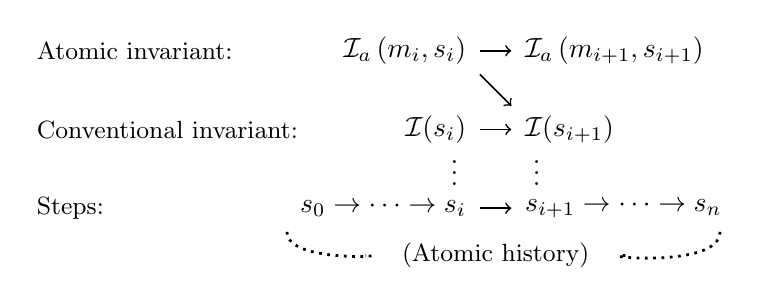
\begin{tikzpicture}
      \node[anchor=west] at (-1.7, 2) {{\small Atomic invariant:}};
      \node[anchor=east] at (4.0, 2) {$\mathcal{I}_a\, (\listof{m_i}, s_i)$};
      \node[anchor=west] at (4.5, 2) {$\mathcal{I}_a\, (\listof{m_{i+1}}, s_{i+1})$};
      \draw [->, line width=0.6pt] (4.05, 2) -- (4.45, 2);
      \draw [->, line width=0.6pt] (4.05, 1.7) -- (4.45, 1.3);

      \node[anchor=west] at (-1.7, 1) {{\small Conventional invariant:}};
      \node[anchor=east] at (4.0, 1) {$\mathcal{I}(s_i)$};
      \node[anchor=west] at (4.5, 1) {$\mathcal{I}(s_{i+1})$};
      \draw [->, line width=0.6pt] (4.05, 1) -- (4.45, 1);

      \node[anchor=east] at (3.9, 0.55) {$\vdots$};
      \node[anchor=west] at (4.6, 0.55) {$\vdots$};

      \node[anchor=west] at (-1.7, 0) {{\small Steps:}};
      \node[anchor=east] at (4.0, 0) {$s_0 \to \cdots \to s_i$};
      \node[anchor=west] at (4.5, 0) {$s_{i+1} \to \cdots \to s_n$};
      \draw [->, line width=0.6pt] (4.05, 0) -- (4.45, 0);

      \node at (4.25, -0.6) {{\small (Atomic history)}};
      \draw [dotted, line width=1pt] (1.6, -0.3) to[out=-90,in=0] (2.6, -0.6);
      \draw [dotted, line width=1pt] (7.1, -0.3) to[out=-90,in=-180] (5.9, -0.6);
    \end{tikzpicture}\\
    \hline
  \end{tabular}
  \caption{Atomic invariants in conventional invariant proof}
  \label{fig-use-atomic-inv}
\end{figure}

The three induction cases ([TSilent], [TIns], and [TOuts]) do not need any special treatment, since each case induces just a single step.
The [TAtomic] case, however, requires coordination with atomic invariants.
In other words, we can employ both conventional/atomic invariants ($\mathcal{I}$ and $\mathcal{I}_a$) to prove the ones for the next state ($s_{i+1}$):
\autoref{fig-use-atomic-inv} explains how to use an atomic invariant $\mathcal{I}_a$ while proving a conventional invariant $\mathcal{I}$ in the [TrsAtomic] case.
The point is that we can employ both $\mathcal{I}(s_i)$ and $\mathcal{I}_a\, (\listof{m_i}, s_i)$ to prove $\mathcal{I}(s_{i+1})$.
For instance, we may want to have an invariant claiming that at most one node of the system has M status at a time.
We will indeed use this invariant in our case studies, although the exact statement is a bit more complex.
The predicate messages defined in \autoref{fig-ex-atomic-invariants} will play a crucial role here, \eg{} the one for \idmsf{8}{rsM} says that $C_1$ and $P$ both have I status, which means that the state transition by $(r_2: C_2.\textrm{st} \leftarrow M)$ preserves the invariant.
We will see more comprehensive uses of predicate messages in our case studies (\autoref{sec-case-study}).
